%% CORREGIR %%%%

%%%%%%%%%% NO OLVIDAR COLOCAR ESTE COMENTARIO CON EL NUMERO DE EJERCICIO %%%%%%%%%%%%%
%%%%%%%%%%%%%%%%%%% EJERCICIO 1 %%%%%%
%%Text bf para negrilla , el \\ es para el salto de linea.
%%El primer \\ hace un espacio en el  texto y el 2 \\ crea otro espacio
\textbf{Ejemplo 1}\newline
Se necesita adquirir un motor para la planta de acabados de una fábrica, en el mercado existen dos marcas de motores que cumplen con las especificaciones técnicas de potencia, velocidad, eficiencia, etc.
La información que desde el punto de vista económico se proporciona, es la siguiente:\\ 
\begin{center}
		\begin{tabular}{|l|l|l|l|}
			
			\hline
			   &                               & A       & B       \\ \hline
			1. & Costo inicial                 & 100.000 COP & 500.000 COP \\ \hline
			2. & Costo mensual de operación    & 5.000 COP   & 10.000 COP \\ \hline
			3. & Años de vida útil             & 5       & 20      \\ \hline
			4. & Valor de salvamento           & 15.000 COP  & 150.000 COP \\ \hline
			5. & Reparación general del año 12 & |-      & 200.000 COP \\ \hline
		\end{tabular}
  \hspace{1cm}
\end{center}

Con una tasa del 2.5 nominal anual mes vencido, hallar la mejor alternativa. \\

\textbf{Solución.}\\



\begin{center}

	\renewcommand{\arraystretch}{1.5}% Margenes de las celdas
	%Creación de la cuadricula
	\begin{longtable}[H]{|c|c|c|}
		%Creamos una linea horizontal
		\hline
		%Definimos el color de la primera fila
		\rowcolor[HTML]{FFB183}
		%%%%% INICIO ASIGNACIÓN FECHA FOCAL %%%%%%%
		%%%%%%%%%% INICIO TITULO
		%Lo que se hace aquí es mezclar las 3 columnas en una sola
		\multicolumn{3}{|c|}{\cellcolor[HTML]{FFB183}\textbf{1. Asignación período focal}}   \\ \hline
		%%%%%%%%%% FIN TITULO
		%%%%% INICIO DECLARACIÓN DE VARIABLES %%%%%%%
		\multicolumn{3}{|c|}{$pf = 0 pav$} \\ \hline
		%Definimos el color de la primera fila
		
		%%%%% INICIO DECLARACIÓN DE VARIABLES %%%%%%%
		%%%%%%%%%% INICIO TITULO
		\multicolumn{3}{|c|}{\cellcolor[HTML]{FFB183}\textbf{2. Declaración de variables}}\\ \hline                                                                                   
		%%%%%%%%%% FIN TITULO
		%%%%%%%%%% INICIO DE MATEMÁTICAS
		$\text{Alternativa A  Alternativa B}$ & $ i= 2,5\% \textit{ pmv }$ & $ \equiv0.34489 \textit{ pav}$\\
		$VP = 100{.}000\text{ COP}$ & $VP = 500{.}000\text{ COP}$ & $n = 5\textit{ pav }$\\
		$VS =  15{.}000\text{ COP}$ & $VS =  150{.}000\text{ COP}$ &  $CPUE =  \text{ COP?}$\\
		$VU =  5 \textit{ años }$ & $VU =  \textit{ años }$ & $m_{1} = 1^2 $\\
		$CMO = 5{.}000\text{ COP}$ & $CMO = 10{.}000\text{ COP}$ & $m_{2} = 1 $\\
		$REP = 200{.}000\text{ COP}$&&\\\hline 
		%%%%%%%%%% FIN DE MATEMÁTICAS
		%%%%% FIN DECLARACIÓN DE VARIABLES
		
		%%%%% INICIO FLUJO DE CAJA
		\rowcolor[HTML]{FFB183}
		\multicolumn{3}{|c|}{\cellcolor[HTML]{FFB183}\textbf{3. Diagrama de flujo de caja}}                                                                                  \\ \hline
		%Mezclamos 3 columnas y pondremos el dibujo
		%%%%%%%%%%%%% INSERCIÓN DE LA IMAGEN
		\multicolumn{3}{|c|}{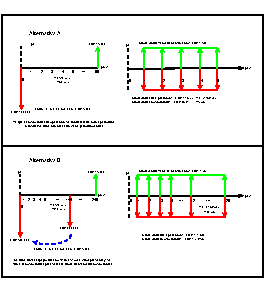
\includegraphics[trim=-5 -5 -5 -5 , scale=2]{10_Capitulo/ejemplos/1/Ejemplo_1.pdf}}                                                                                         \\ \hline
		%%%%%%%%%%%%% FIN INSERCIÓN DE IMAGEN
		%%%%%FIN FLUJO DE CAJA



		%%%%% INICIO DECLARACIÓN FORMULAS
		%%%%%%%%%%% INICIO TITULO
		\rowcolor[HTML]{FFB183}
		\multicolumn{3}{|c|}{\cellcolor[HTML]{FFB183}\textbf{4. Declaración de fórmulas}}                                                                                    \\ \hline
		%%%%%%%%%%% FIN TITULO
		%%%%%%%%%%% INICIO MATEMÁTICAS

		\multicolumn{3}{|c|}{$(1+i_{1})^{m1}=(1+i_{2})^{m2} \text{ Equivalencia de   tasas}$}\\ 
		\multicolumn{3}{|c|}{$VP=R\frac{1-(1+i_{1})^{-n}}{i_{2}} \text{ Valor presente serie uniforme vencida}$}\\ 
		\multicolumn{3}{|c|}{$VF=R\frac{1-(1+i_{1})^{n}}{i_{2}} \text{ Valor futuro serie uniforme vencida}$}\\
		\hline
		%%%%%%%%%% FIN MATEMÁTICAS
		%%%%%% INICIO DESARROLLO MATEMÁTICO
		\rowcolor[HTML]{FFB183}
		%%%%%%%%%%INICIO TITULO
		\multicolumn{3}{|c|}{\cellcolor[HTML]{FFB183}\textbf{5. Desarrollo matemático}}                                                                                      \\ \hline
		%%%%%%%%%% FIN TITULO
		%%%%%%%%%% INICIO MATEMÁTICAS

		Alternativa A & \multicolumn{2}{c|}{Alternativa B}\\
		Costo mensual de operación anual & \multicolumn{2}{c|}{Pago año 12 en valor presente} \\
		${5{.}000*\frac{1,025^{12}-1}{0,025} = 68{.}978 COP}$ & \multicolumn{2}{c|}{${VP=200	{.}000(1,34489)^{-12} =  5{.}712}COP$}\\
          \text{cuota anual operación años }& \multicolumn{2}{c|}{}\\
		Cuota anual costo inicial & \multicolumn{2}{c|} {Valor inicial + Valor presente pago año 12}\\
		${R=\frac{100{.}000}{\frac{1-(1,34489)^{-5}}{0,34489}} = 44{.}633}COP $  & \multicolumn{2}{c|}{$500{.}000COP + 5{.}712COP = 505{.}712COP$}\\
		Cuota anual valor salvamento &\multicolumn{2}{c|} {Cuota anual costo inicial}\\
		${R=\frac{15{.}000}{\frac{(1,34489)^{5}}{0,34489}}} = 1{.}522COP $ & \multicolumn{2}{c|}{${R=\frac{505{.}712}{\frac{1-(1,34489)^{-20}}{0,34489}} = 174{.}882 }COP$}  \\ 
		&\multicolumn{2}{c|}{Cuota anual valor salvamento}\\ 
		&\multicolumn{2}{c|}{${R=\frac{150{.}000}{\frac{(1,34489)^{20}}{0,34489}} = 138COP }$}\\ 
		&\multicolumn{2}{c|}{Costo mensual operación anual}\\ 
		&\multicolumn{2}{c|}{${10{.}000*\frac{1,025^{12}-1}{0,025} = 137{.}956 }COP$} \\ 
		CPUE alternativa A & \multicolumn{2}{c|}{CPUE alternativa B} \\ 
		$CPUE_{A} = 1.522-44.633-68.978$ &\multicolumn{2}{c|}{$CPUE_{B} = 138-174.882-137.956$}\\ 
		$CPUE_{A} = -112.089 COP$ &\multicolumn{2}{c|}{$CPUE_{B} = -312.700COP$}\\ 
		\hline 
		%%%%%%%%%% FIN MATEMÁTICAS
		%%%%%% FIN DESARROLLO MATEMÁTICO

		\rowcolor[HTML]{FFB183}
		\multicolumn{3}{|c|}{\cellcolor[HTML]{FFB183}\textbf{6. Respuesta}}    \\ \hline

		\multicolumn{3}{|c|}{El CPUE para la adquisición de un motor de la marca A es de  -112.089COP} \\ \hline
	\end{longtable}
	%Se crean dos lineas en blanco para que no quede el siguiente texto tan pegado
	%\newline \newline
\end{center}
%%%%%%%%%%%%%%%%%%%%%%%%%%FIN EJERCICIO X %%%%%%%%%%%%%%%%%%%%%%%%%%%